\chapter{Interdisciplinary tree disease epidemics}
\label{chapter2:litreview} 

Understanding modern-day tree disease epidemics requires a holistic, interdisciplinary scientific 
approach, made possible only by the convergence of numerous scientific fields. 
Consequently, this Chapter reviews several key modelling themes.

Typically, models of tree disease aim to help design effective control policies and inform policymakers.
Well-informed policymakers can then help to maintain tree health in rural, urban and commercial environments. 
Although myriad environmental, biological and anthropomorphic factors complicate the scientific understanding 
and thus effective disease control. 

The review begins by narrating early historical developments in human and botanical epidemiology before presenting
a variety of present-day modelling frameworks. After introducing the mainstream paradigm of plant-based epidemic models,
an inspection of dispersal, thresholds, and epidemic control follow naturally. In addition, several host data sources 
in Great Britain are presented. Finally, the Chapter ends with an ash dieback case study, reflecting the multi-faceted 
difficulties posed by a recent emergent epidemic.

\section{Historical perspectives}

Historically, the fields of plant pathology and mathematical epidemiology existed in different spheres.
Plant pathology researchers furthered biological understanding of pathogen growth (e.g. \cite{doi:10.1146/annurev.py.01.090163.000245}), not predictive mathematical theories.
Although, pioneering discoveries in mathematical epidemiology permitted a more quantitative treatment of botanical diseases. 
In particular, the seminal $SIR$ model of \cite{kermack-model} 
provided a foundation to examine plant-based epidemics mathematically.

\subsection{Standard $SIR$}

The \cite{kermack-model} (K \& M) model involves three compartmentalised fields, 
susceptible $S(t)$, infected $I(t)$ and removed $R(t)$.
Each field models the evolution of a closed population of size $N$, where $N = S(t) + I(t) + R(t)$. 
A coupled system of ODEs then follow:
\begin{align}
\label{eq:SIR-model1}
    &\frac{dS}{dt} = -\beta SI \\
    &\frac{dI}{dt} = \beta SI - \mu I \\
    \label{eq:SIR-model3}
    &\frac{dR}{dt} = \mu I
\end{align}
where the term $\beta S I$ dictates the flow of susceptible hosts into the infected compartment according 
to the rate $\beta$. Likewise, $\mu I$ controls the transition of infected hosts into the removed compartment
through a removal rate $\mu$. Figure \ref{fig:SIR-vs-plank}(a) illustrates the coupled $SIR$ system for 
fixed $\mu$ and four values of $\beta$.

The coupled differential system of Equations (\ref{eq:SIR-model1}-\ref{eq:SIR-model3}) rely on several assumptions, including:
1) a closed population with no births or deaths 2) no exposed/incubation period 3) lifetime immunity following recovery
4) mass action population mixing, where contact mixing rates between individuals in $S$ and $I$ are proportional 
to the number of individuals in either field.

Today, countless articles have relaxed these assumptions to extend the standard $SIR$ framework\footnote{
Indeed, following the COVID-19 pandemic, $SIR$-type models remain an active field of research 
and dominate present-day epidemic literature \cite{atkeson2020using}.}.
Nevertheless, a keystone result emerged from Equations (\ref{eq:SIR-model1}-\ref{eq:SIR-model3}), namely 
the existence of a critical epidemic threshold, captured through either:
\begin{align}
    \label{eq:R0-SIR}
    & R_0 = \frac{\beta}{\mu}\\
    \label{eq:R0-effective}
    & R_e = \frac{S(t)}{N} \frac{\beta}{\mu}
\end{align}
where $R_0$ and $R_c$ are referred to as the basic and effective reproduction numbers, respectively.
Following the introduction of one infected host at $t=0$, $N\sim S(0)$ and 
we have $R_e=\big((N-1)/N\big) \beta / \mu$. Therefore, in the limit of a large population at $t=0$, 
$\big((N-1)/N\big)$ approximates unity and $R_e = R_0$, otherwise $R_e=\big(S(t)/N\big) R_0$.

Both quantities $R_0$ and $R_e$ describe an epidemic threshold, though $R_e$ captures a threshold in the face
of a declining susceptible population by including the ratio $S(t)/N$.
Equation \ref{eq:R0-effective} defines a critical threshold by the simple criterion\footnote{
For a more comprehensive mathematical proof of $SIR$
model thresholds, the reader is directed towards \cite{weiss2013sir}}:
1) when $R_e > 1$, then $I(t)$ rises sharply, culminating in an epidemic before declining in the absence of newly
infected hosts
2) if $R_e \leq 1$, then $I(t)$ quickly declines to zero as $t\rightarrow 0$ and the outbreak subsides.


\subsection{Logistic growth}

The seminal work of \cite{van2013plant} firmly established ties between plant pathology and 
mathematical epidemiology.
Fundamentally, Van der Plank equated the growth of plant pathogens (or `inoculum') to logistic growth of the form:
\begin{equation}
    \label{van-plank}
    \frac{dI}{dt} = rI(1 - I)
\end{equation}
where $r$ describes the rate of pathogen growth and $I$ reflects the proportion of infected tissue.
In Equation \ref{van-plank}, the amount of infected tissue $I$ snowballs at first, 
in proportion to the amount of inoculum. Then, as time passes and $I$ grows, $(1-I)$ approximates zero, 
and the system plateaus as all susceptible tissue becomes infected.
The essential model behaviour is shown in Figure \ref{fig:SIR-vs-plank}(b) over $10$ values growth rates $r$.
From Equation \ref{van-plank}, a simple method to determine the rate $r$ follows:
\begin{equation}
    \label{eq:van-plank-r}
    r =\frac{1}{t_2 - t_1} \log \Big(\frac{I_2}{1 - I_2} - \frac{I_1}{1 - I_1}\Big)
\end{equation}
where $I_1$ and $I_2$ are the proportions of infected tissue at times $t_1$ and $t_2$ respectively\textemdash 
see \cite{van2013plant} Chapter 3. Importantly, both $I_1$ and $I_2$, and by extension the infection rate $r$,
are measurable in laboratory conditions. 
In Equation \ref{van-plank}, newly infected tissue becomes infectious immediately following infection.
Realistically, infectious tissue (and symptom expression) takes time to develop, described by an `incubation period'.
Accordingly, Van der Plank adapted Equation \ref{van-plank} to a delay differential equation (DDE):
\begin{equation}
\label{van-plank-incubation}
    \frac{dI_t}{dt} = RI_{t-p}(1 - I_{t})
\end{equation}
where $I_t$ and $I_{t-p}$ describe the infectious tissue at times $t$ and $t-p$ and $p$ is the incubation period. 
Hence, infectious tissue grows in response to the factor $R I_{t-p}$, and saturates
according to the logistic term $(1 - I_t)$. The parameter $R$ now describes pathogen
growth at step $t-p$, as opposed to $r$ that describes the spread of disease at step $t$, leading to the ratio:
\begin{equation}
    \frac{R}{r} = \frac{x_t}{x_{t-p}}
\end{equation}
\begin{figure}
     \centering
     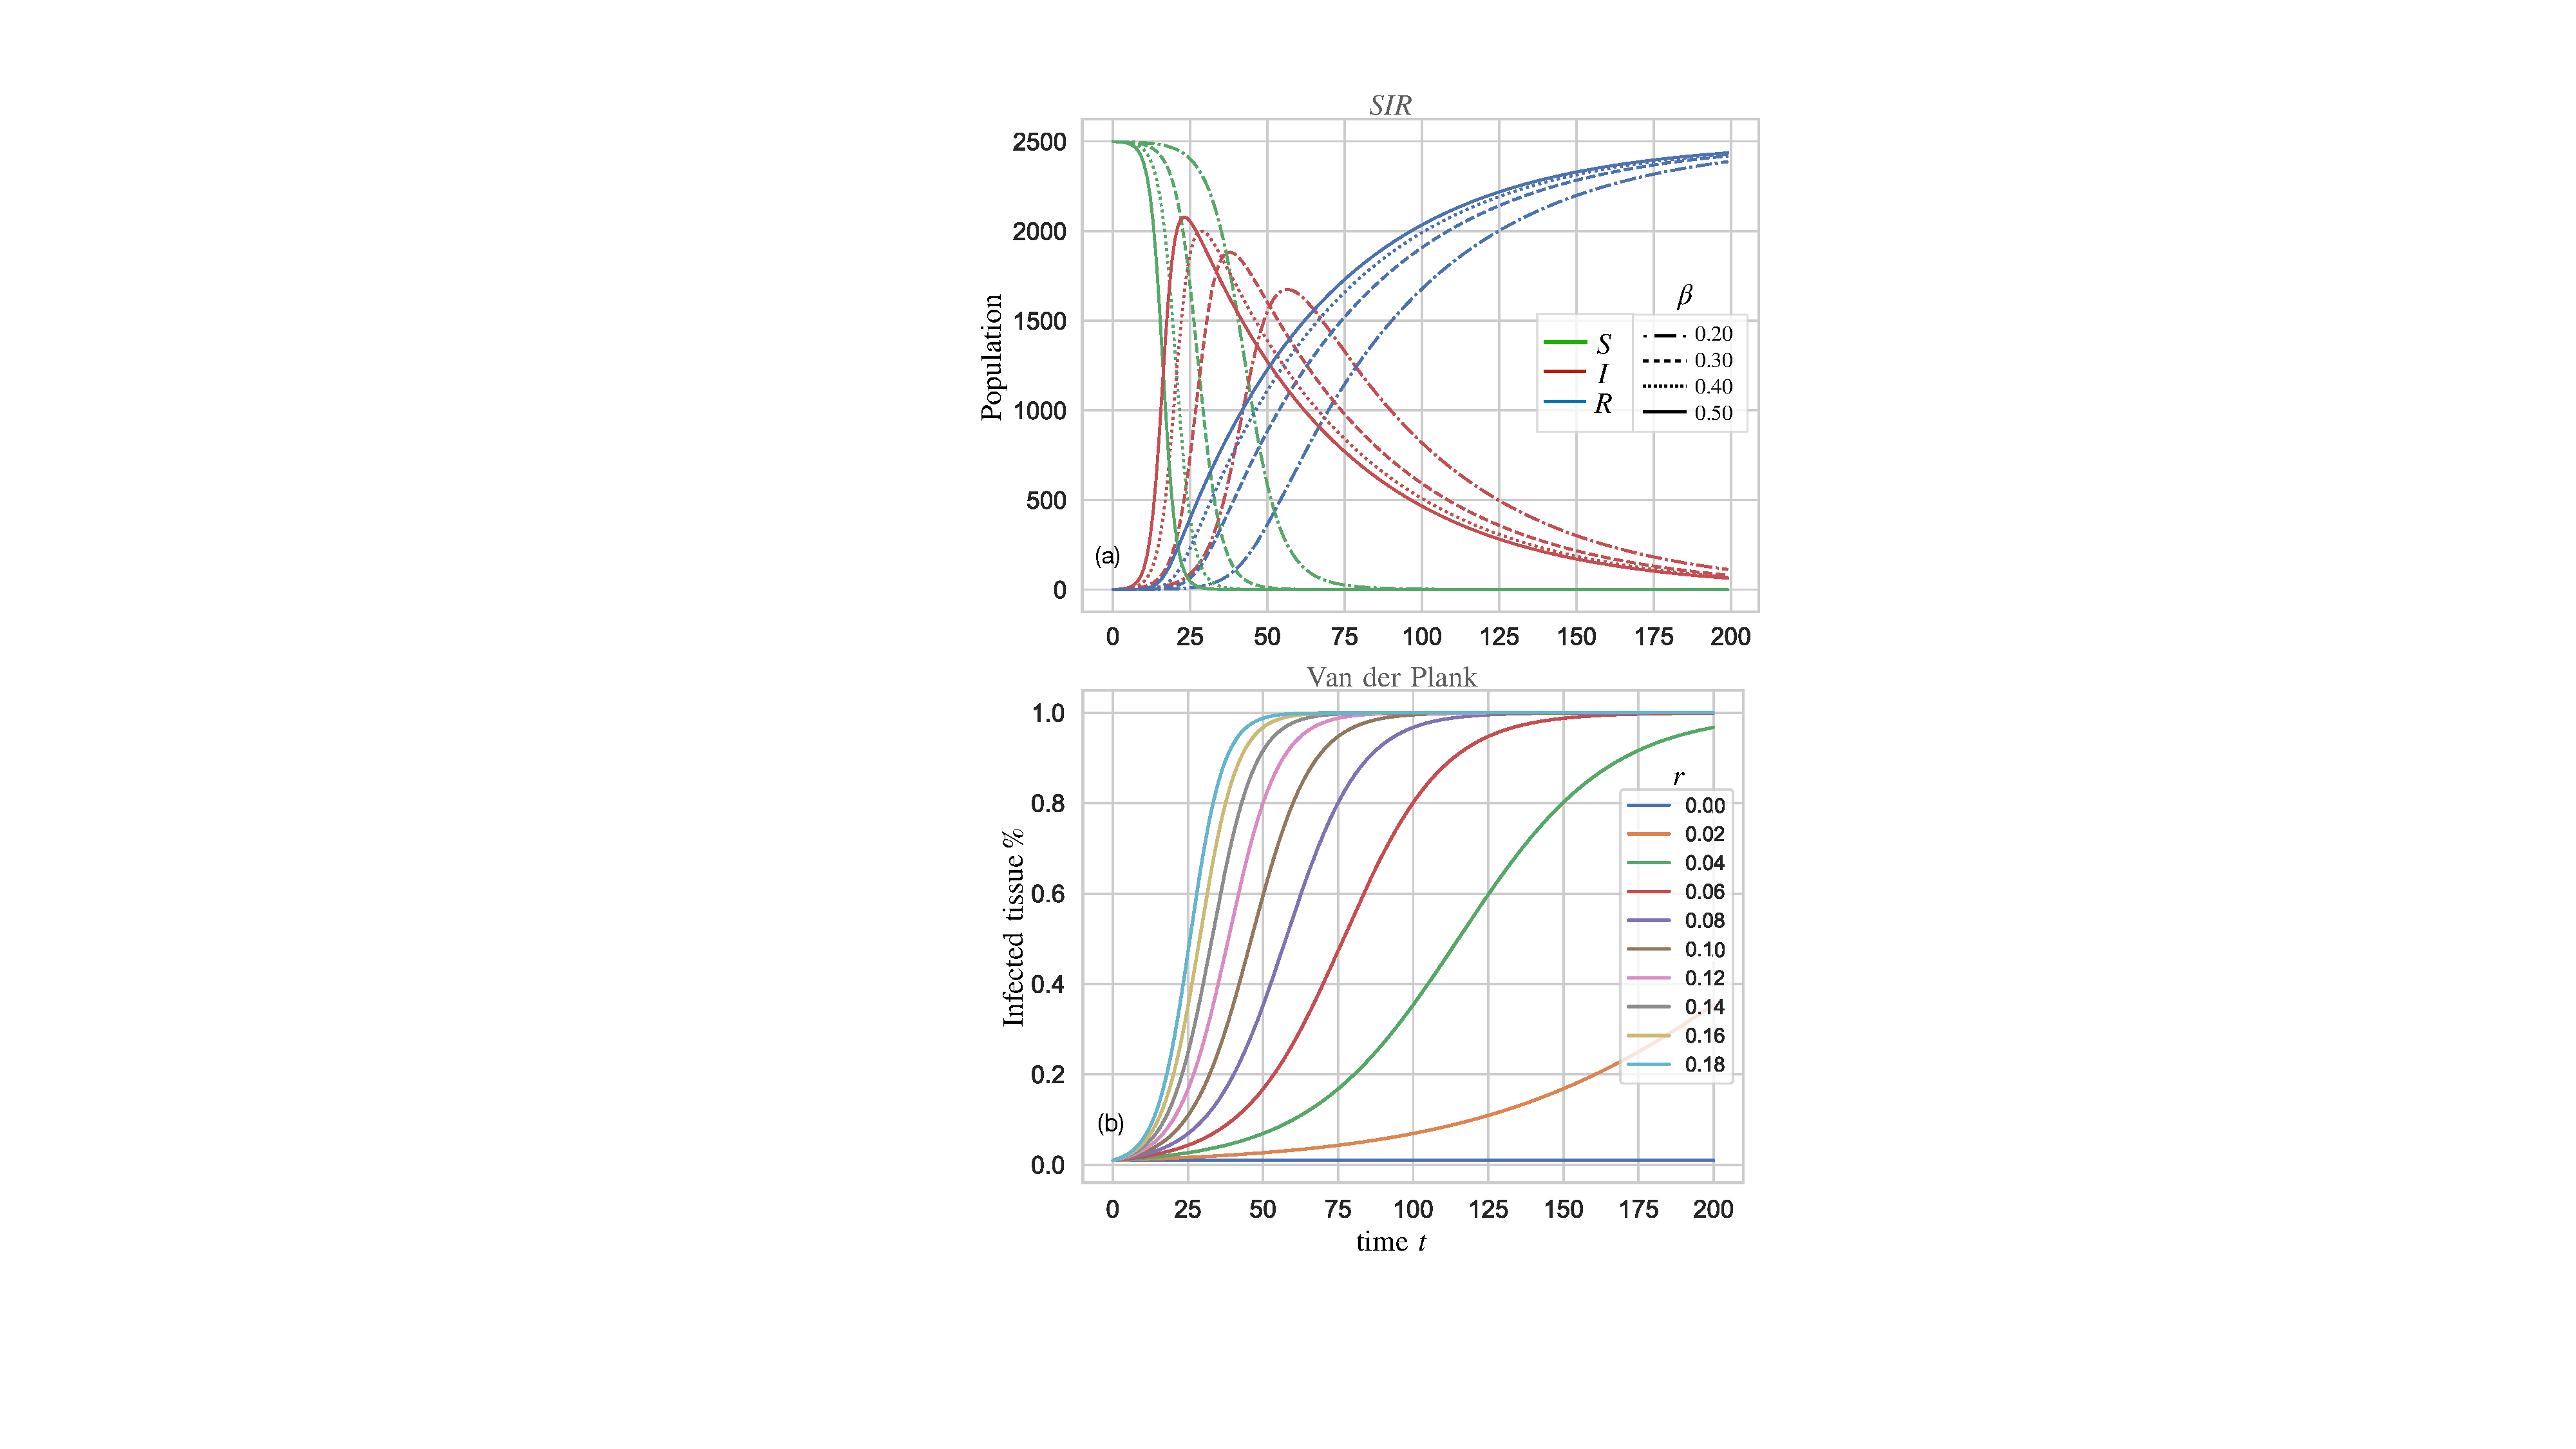
\includegraphics[scale=0.55]{chapter2/figures/SIR-vs-Plank.pdf}
     \caption{(a) The $SIR$ model as presented by \cite{kermack-model} is shown for fixed removal rate $\mu = 0.20$ and variations of $\beta$. 
                  The coupled system of ODEs can be solved numerically with Euler's method. Here, simulations begin with 
                  $2500$ susceptible and one infected individuals, and evolve for $t=200$ steps.
                  (b) The logistic growth model \cite{van2013plant} used to describe the growth of infected plant material.
                  Simulations are numerically computed with a forward-time finite difference method for $10$ different growth rates $r$.
       } 
     \label{fig:SIR-vs-plank}
 \end{figure}
where $r$ represents an `apparent' infection rate (measurable in laboratories from Equation \ref{eq:van-plank-r}),
and $R$ denotes the `basic' infection rate. As Plank explained, one usually seeks
to determine $R$ from the constant $r$. Assuming that $r$ indeed stays constant over the epidemic:
the basic infection rate $R$ must decrease as $x_t/x_{t-p}$ gets progressively smaller as $x_{t-p}\rightarrow x_t $.
At this point, the basic infection rate $R$ begins to resemble the effective reproduction ratio $R_e$
from Equation \ref{eq:R0-effective}. 

Equation \ref{van-plank-incubation} describes a system where
infections incubate for a period $p$ before inducing the growth of more infectious plant tissue.
However, it does not describe the infectious period (where infected tissue remains before becoming epidemiologically inert),
which lead Plank to extend Equation \ref{van-plank-incubation} to:
\begin{equation}
\label{van-plank-infectious-p}
    \frac{dI_t}{dt} = R_c(I_{t-p} - I_{t-i-p})(1 - I_{t})
\end{equation}
where $R_c$ is the basic infection rate `corrected' for removals and $i$ is the infectious period.
In this DDE, a unit of latently infectious tissue starts becoming infectious after $p$ steps, and stops becoming infectious $i$ steps.
More formally, as $I_{t-i-p} \rightarrow I_{t-p}$, the rate of infectious tissue growth approaches zero, $dI_t/dt \rightarrow 0$.

\subsection{Contrasting approaches}

The $SIR$ model does not include an incubation period, and therefore differs from the delayed differential formulation 
of Equation \ref{van-plank-infectious-p}. Nonetheless, the compartmentalised approach is easy to extend, leading to an 
$SEIR$ system:
\begin{align}
\label{eq:SEIR-model1}
    &\frac{dS}{dt} = -\beta SI \\
\label{eq:SEIR-model2}
    &\frac{dE}{dt} = \beta SI - \gamma E\\
    &\frac{dI}{dt} = \gamma E - \mu I \\
    \label{eq:SEIR-model3}
    &\frac{dR}{dt} = \mu I
\end{align}
where Equation \ref{eq:SEIR-model2} describes the population of latently (or exposed) infected hosts.
Susceptible hosts transition into the exposed compartment at the same rate as before, namely $\beta SI$, but now have an
exponentially distributed latency period of $\gamma^{-1}$ before transitioning into $I$.

Both Equations \ref{eq:SEIR-model1}-\ref{eq:SEIR-model3} and Equation \ref{van-plank-infectious-p} outline similar systems,
though infected tissue in Equation \ref{van-plank-infectious-p} remains infectious for precisely $i$ units.
This contrasts with the exponentially distributed exposed lifetime implicit within Equation \ref{eq:SEIR-model2}.
Nevertheless, \cite{segarra2001epidemic} illustrated how Plank's DDE and the $SEIR$ system are both special cases of
the $SIR$ model proposed by \cite{kermack-model}, when the $SIR$ model incorporates a sporulation function, $\phi(\tau)$. 
The sporulation function appropriately models spore production in plant pathogens. 
In particular, if $\phi(\tau) = 0$ for small $t$, $\phi(\tau)$ can model incubation periods. 
Similarly, if $\phi(\tau) = 0$  for large $t$, we recover an infectious period. 
More recently, \cite{time-varying-infectivity} simplified the analysis of \cite{segarra2001epidemic}, showing that 
both Plank's DDE and the $SEIR$ model can be recovered with an $SE_nI_mR$ model.
In an $SE_nI_mR$ framework, both $n$ and $m$ represent an arbitrary number of distinct exposed and infectious compartments:
\[
    S\rightarrow E_1 \rightarrow E_2 \rightarrow ... \rightarrow E_n \rightarrow I_1 \rightarrow I_2 \rightarrow ... I_m
\]
Trivially, the $SEIR$ model is recovered when $n=1$ and $m=1$. However, when $n,m \rightarrow \infty$,
\cite{time-varying-infectivity} demonstrated that we recover an expression equivalent to the DDE in Equation \ref{van-plank-infectious-p}.
Despite the sameness of both DDE and $SEIR$ formulations, the overarching theme of modern epidemiology is overwhelmingly compartmentalised,
owing to the increased flexibility and easier analysis of compartmental models.

\subsection{Progressive botanical epidemiology}

After \cite{van2013plant} moved the field of botanical diseases into a more quantitative discipline,
theoretical investigations (alongside the adoption of computer simulations) characterised the next few decades.
Plank's DDE was applied to numerous pathosystems, halo blight in beans \cite{doi:10.1111/j.1744-7348.1979.tb06527.x} 
and grape powdery mildew \cite{sall1980epidemiology} to name a few. In particuar, \cite{sall1980epidemiology} adapted Plank's
logistic approach to include a time-varying infection rate $r(t)$. Moreover, diverse mathematical techniques, 
including multiple  regression analysis, were incorporated into mainstream plant epidemiology \cite{butt1974multiple}. 
Subsequently, \cite{zadoks1979epidemiology} consolidated various early mathematical models of plant disease 
alongside \cite{jeger1984use}.

Developments in computing compounded advances in plant epidemiology through this period. 
Improved accessibility and computer architectures permitted faster calculations and more intensive models. 
The first epidemic simulator (EPIDEM) written in FORTRAN IV came by \cite{waggoner1969epidem}. 
EPIDEM modelled the fungi `Alternaria solani' spreading through infected potato and tomato leaf tissue under different environmental conditions. 
    
An interesting early simulator (EPIMUL76) developed by \cite{zadoks1977role} adapted Van der Plank's logistic growth model into a spatio-temporal framework of two spatial dimensions. 
EPIMUL76 simulated the spread of disease on a two-dimensional domain, subdivided into $20\times 20$ host units referred to as `compartments', that took place inside a computer with $128\mathrm{K}$ of memory.
Arguably, subdividing the domain into separate compartments could be considered as an
agent-based model. 

In their analysis, \cite{zadoks1977role} alluded to the problem of scale in plant disease, as spatial scales
were conceptualised as microscale ($\leq 1\mathrm{m}$), mesoscale ($10^2\mathrm{m}$) and macroscales ($10^6\mathrm{m}$). 
In this picture: microscales ranged from plant leaves to individual plants, the mesoscale as crop fields, and the macro scale
as large regional expanses over a country-wide scale. Moreover, the probability of dispersal between infected hosts assumed a
Gaussian distribution\textemdash in contrast to \cite{doi:10.1146/annurev.py.06.090168.001201}.
In general, the ability to simulate more intricate models grew in proportion to the amount of computer memory available.
For a review of early plant disease simulators, see \cite{doi:10.1146/annurev.py.23.090185.002031}.

\section{Epidemic stochasticity}

The spread of disease inherently takes the form of a stochastic process, whereby an epidemic unexpectedly arises and quickly cease, seemingly out of the blue. In order to capture the spread of disease, stochastic effects cannot be overlooked... 

\begin{itemize}
    \item Motivate this Chapter based on the determinism of \cite{kermack-model} and \cite{van1999pandemics}
    \item Explain why stochastic is an essential part of epidemics
    \item How do you collect results of a stochastic model ? Ensemble averaging
\end{itemize}

\section{Percolation: from forest fires to epidemics}
\label{section:lit-rev-perc}

\begin{itemize}
    \item Motivate percolation based on the stochastic arguments listed above 
    \item articulate that percolation has a spatial context 
\end{itemize}

The original formulation of percolation theory was first used to describe properties of a fluid and the bonds which form between molecules \cite{perco_origin} (the reader may jump to \ref{fig:ch3-perc-invariance} for an account of percolation). The problem was posed on a graph\textemdash illustrated in terms of vertices and edges. However re-interpretations were subsequently put forward by physicists studying material sciences, naturally on a lattice. \cite{Essam_1980}. The attractive feature of this new paradigm was that percolation demonstrated a phase-transition. Thus, percolation could be treated with scaling theory used in the study of critical-phenomena. Accordingly, early work rigorously ensued to map out the behaviour of percolation around criticality in terms of critical exponents \cite{STAUFFER19791}. 

Different flavours of percolation models, such as, site or bond percolation were described to model different processes. Percolation proved a convenient theory and various phenomena including, gelation, magnetism and telecommunications were described \cite{trove.nla.gov.au/work/26493727}. Interestingly, forest fires were also applicable to a description within percolation theory \cite{MacKay_1984}. This was a short conceptual jump from time-dependant percolation used to study the growth of crystals \cite{Family_1985}. 

A fire spreading through a population of trees is not to dissimilar to a disease spreading through a population. This lead to a general epidemic-formalisation within percolation-based framework when \cite{pub.1059067807} argued that epidemics were in the same universality class as percolation. It is alluring to remark how modelling the same processes with different microscopic interactions (e.g. different lattice geometries) lead to the macroscopic behaviour should they have the same universality class\textemdash see Chapter \ref{fig:ch3-perc-invariance} for more information.

Beginning with a simple $SIR$ framework put forward by \cite{kermack-model}, the field of epidemiology was already well established around the time percolation theory was conceived \cite{baily1975mathematical}. In particular, initial assumptions about population mixing could be relaxed with more elaborate spatial-contact models, naturally, percolation theory could serve as a useful tool when developing spatially-structured epidemic models.

A fractal-like pattern of epidemics was observed by \cite{GRASSBERGER1986273}, shown in Figure \ref{fig:1d_perc_basis}. Parsimoniously describing Figure \ref{fig:1d_perc_basis}, lighter grey sites represent removed individuals, black sites indicate actively infected sites and white sites indicate unaffected sites. All lattice sites in the bottom row were initially infected and the infection can be seen to propagate from the bottom up. The lattice was initialised at the critical-density $p\sim p_c$ culminating in a fractal-like pattern. \cite{GRASSBERGER1986273} did not attribute the hosts of this model to be trees, but instead a general host-population with very low mobility. Local interactions between hosts and infected were elucidated as vast simplifications and long-range interactions (following a power-law) were discussed\textemdash we shall see how these ideas form a important component of modelling tree disease.

\begin{figure}
    \centering
    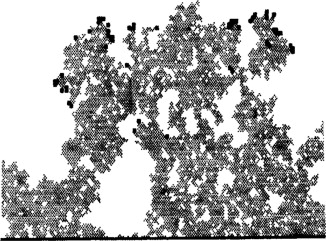
\includegraphics{chapter2/figures/perc1.jpg}
    \caption{A space-time representation of an epidemic spreading at the critical threshold. The spatial (horizontal) and time (vertical) axis show self-similar propagation of diseased individuals in grey, produced by \cite{GRASSBERGER1986273}}
    \label{fig:1d_perc_basis}
\end{figure}

The behaviour of percolation-based epidemic models continued (e.g. \cite{pub.1060474189, pub.1059069981}) to be investigated with various methods such as renormalisation-groups and Monte-Carlo, the critical exponents were found along with phase transition graphs characterising epidemic (super-critical) or extinction (sub-critical) regimes. The properties of both epidemics and forest fire percolation models were studied together in \cite{pub.1052857560}, highlighting their similarity.

The first ecological application came in \cite{pub.1031591030} where forest fire (and epidemic) percolation models were adapted in order to study landscape disturbances. Broadly speaking, landscape disturbances constitute a broad array of physical process which lead to a rapid ecological change, this could include invasion of pests, climate-change and fire.

% \textemdash \cite{GRASSBERGER1983157} <- reference for early considerations towards percolation as a model for tree diseases and percolation
% \textemdash \cite{SANDER2002293}, read and get more info + research links

\section{Spatially-explicit epidemic models}
\label{ch2:lit-rev-compartmentalised-models}
Compartmentalised models are the dominate theme in epidemiological modelling...

% 1 - early work that decomposed KMc model 
\cite{segarra2001epidemic}

% 2 - describe how plank model can be represented in terms of a compartmentalised model
The authors of \cite{time-varying-infectivity} demonstrated that different sporulation functions can be derived from a more general class of $SEmInR$ models. 
Sporulation functions can then be used to describe lifetime of transitions between $E\rightarrow I$ along with the time-dependency of infectivity rates in the transition $S\rightarrow E$. 

% In his seminal work, van der Plank \cite{van2013plant} considered a latency and infectious period, with a constant rate of infection while infectious; this model is represented by the equation:
% \begin{equation}
% \label{eq:plank-model}
%     \frac{dI(t)}{dt} = R\big(I(t - p)  - I(t - p - i)\big)\big(1 - I(t)\big)
% \end{equation}

% where $p$ and $i$ are constant latency and infectivity periods and $R$ is the corrected infection rate (i.e. including host demography). Equation \ref{eq:plank-model} is seldom used in contemporary literature, owing to the difficulty in analytically solving its time-delay \cite{madden2006botanical}. However, it provides a simple basis to understand time-varying infectivities. 

% Later, \cite{time-varying-infectivity} demonstrated that sporulation can be decomposed into a suite of $SEIR$-like models. Specifically, the authors of \cite{time-varying-infectivity} demonstrated that both compartmentalised $SEIR$ models and the plank formulation can be decomposed into a $SEmInR$ model i.e. where transitions follow $S\rightarrow E_1, E_2,.., E_m \rightarrow I_1, I_2, ..., I_n \rightarrow R$.
% By taking suitable limits of $n$ and $m$ the plank and $SEIR$ models can be recovered. 


\subsection{Lattice-based modelling}
Lattice-based models have been used to describe the spread of disease in many contexts, such as the spread of malaria, the bubonic plague and the spread of tree disease...

% \textcolor{red}{
% \begin{itemize}
%     \item Spatial SIR model
%     \item Agent-based modelling
%     \item A good place to talk about Percolation models
%     \item \textcolor{red}{Murray}: travelling waves that do not change shape
% \end{itemize}}

\subsection{Dispersal}
\label{ch2:dispersal}
One of the key features that distinguish tree disease from human-based disease is dispersal. The dispersal of a pathogen may take many forms..
% \begin{itemize}
%     \item The importance of dispersal
%     \item How is dispersal treated mathematically ?
%     \item What type of dispersal kernels have been studied?
%     \item What parameter-values have been inferred ?
%     \item How long-range can dispersal be ? Talk about long-range inter-Continental dispersal
%     \item see \cite{nathan2012dispersal} for a review of dispersal kernels
% \end{itemize}

\subsection{The role of scale}
% WORK IN PROGRESS
The role of scale is crucial to describing the spread of tree-based disease...
% \begin{itemize}
%     \item The spatial aggregation of vegetation, how does clustering look on different spatial resolutions ?
%     \item Spatial scale in dispersal ? What does this mean for disease gradients ?
%     \item  \cite{https://doi.org/10.1111/jbi.13642}
%     \item  \cite{pautasso2013european}, search for 'modelling' in this review paper. It contains references to LDD models.
%     \item LDD is an important factor of the scale of spread. Long distance dispersal has been considered for many biological processes including seed and pollen dispersal \cite{baguette2012dispersal, levin2003ecology}.
%     \item LDD is highly stochastic \cite{nathan2006long}
%     \item \cite{wingen2013long} demonstrated how host heterogeneity and distance between patches can...
%     \item traditional model of plant disease consider a wave-like spread of disease, a biological wave-like phenomena, that spreads from region to region (CITATIONS...).
%     However, this is not the case, as demonstrated by \cite{mundt2009aerial}. Epidemic fronts and disease gradients can range over multiple scales. The spread of disease through plant-based populations is thus, a multi-scale problem.
%     \item indeed, fungal spores can disperse over large distances, as confirmed by modelling work \cite{shaw2006assembling} 
% \end{itemize}

\section{Modelling landscape-level epidemics}

Modernity has witnessed the spread of tree-based epidemics at the regional, country and continental level. 'landscape-level'

\subsection{The Metapopulation model}

% \begin{itemize}
%     \item this variation in epidemic outcome from variants of environmental factors was likened to the metapopulation used in ecology and population dynamics in order to describe environment `patchiness'
%     \item variability in the host landscape was considered and recognised as important, the patchiness of a landscape lends itself well to a metapopulation model
%     \cite{doi:10.1098/rstb.1986.0072}
%     \item \cite{large-scale-control}
% \end{itemize}

\subsection{Network Modelling}

Network models are useful to describe the spread disease of human-based trade and transport of infectious trees...

% \textcolor{red}{
% \begin{itemize}
%     \item What paradigm do network models suit?
%     \item Human trade and transport and networks 
%     \item plant-to-plant interactions and networks ? 
%     \item give examples of how network models have been used in the literature
%     \item review \cite{doi:10.1098/rsif.2005.0051}
% \end{itemize}}


\section{Thresholds in plant-based disease}

A key theme in the spread of tree-disease, and disease in the broadest sense, can be understood through a threshold...
% \textcolor{red}{
% \begin{itemize}
%     \item What was the first paper to use this term ? Give mini-historical recount
%     \item What is Invasion and persistence ? Give examples of papers and results in literature 
%     \item The importance of thresholds
%     \item Where does this number come from and why is \textbf{}this an important number ?
%     \item How can one define $R_0$ ? Talk about how the there are different ways to calculate it e.g. next-generation operator 
%     \item Survey what results have been obtained in the literature using $R_0$
% \end{itemize}}

\subsection{The basic reproduction number}
\label{ch2:R0}
The basic reproduction number, denoted by $R_0$, can be seen to arise in the study of population dynamics and demographics to categorize offspring \cite{heesterbeek2002brief}. In the study of epidemics, $R_0$ was adapted in order to categorize the number of infectious offspring and is widely agreed to be the most important and informative parameter. The basic reproduction number can be derived from the $SIR$ model \cite{kermack-model}, and from it, we can see how a likely disease is to spread though a population. Numerous definitions of $R_0$, and methods of determination, have been proposed in the literature resulting in confusion and multiple $R_0$ values for one pathogen \cite{delamater2019complexity}. However, a common definition states:

\textit{The expected number of secondary infections that result from one infected individual, over it's entire infectious lifetime, in a completely susceptible population.}

here, the infectious life-time is the total amount of time an individual remains infectious. The individuals infectious status will culminate in either recovery or death. Importantly, from $R_0$ a threshold can be determined which dictates whether or not the disease will spread through large parts of the population. That is, if $R_0>1$ an \textit{epidemic} will result, otherwise the spread of disease will likely halt. The value of $R_0$ can be determined from different methods\footnote{Common approaches include, the survival function, next-generation operator and estimation from epidemiological data \cite{perspectives-on-r0}} and from it many surrogate parameters can be calculated which leads to confusion \cite{diekmann2010construction}.

The basic reproduction number is used extensively by researchers wishing to understand the spread of disease through human populations. In the study of plant-based disease however, the basic reproduction number has attracted far less attention despite being a convenient parameter from which a threshold can be derived. Thresholds are of great importance to understand epidemics in plant-based populations. A threshold criteria similar to the $R_0$-threshold was first introduced by \cite{van2013plant} in the logistic growth model. However, the logistic-growth based threshold was a vast simplification and had limitations in accurately predicting the threshold for growth and spread \cite{onstad1992evaluation}.

The basic reproduction number $R_0$ was studied by \cite{gubbins2000population} in order to understand thresholds in plant-parasite \textit{pathosystems}. A plant-host under attack from a parasite may respond to the \textit{parasite load} with either the promotion or inhibition of susceptible tissue, see \cite{gilligan1997analysis} for further details on this mechanism. In order to model this problem, \cite{gubbins2000population} used a system of three linked differential equations describing the density of susceptible hosts, infected hosts and the primary source of inoculum\footnote{\textemdash here, inoculum is a general term that refers to any part of the parasite that, when in contact with the plant, may induce disease \cite{agrios2005chapter}}. Transmission of inoculum could occur through a dual source, that is, through primary or secondary pathways. Local stability analysis on the linked equations lead to various $R_0$ values, and subsequently threshold criteria, dependant on the functional form assumed by the host-response.\\

\subsection{Invasion and Persistence}
\label{ch3:invasions_and_persistence}
When calculating thresholds, the spatial structure of the host population cannot be overlooked. A study conducted by \cite{park2001invasion} considered how spatial heterogeneity effects the dynamics of plant-parasite interactions and derived the basic reproduction number for a spatially structured host population. The density of susceptible and infected hosts were comparatively examined with deterministic and stochastic model variants. The host population in \cite{park2001invasion} consisted of \textit{patches}, which in reality could be either a single host, field or region of land. Inside each patch, the \textit{within-patch} dynamics were governed by a basic reproduction number, $R_p$. If $R_p > 1$ the parasite could survive and reproduce locally or otherwise die. The infection could jump between different patches via a longer-range interaction, set by a coupling strength. Patches were locally coupled together in a neighbourhood and the infection could jump between neighboring patches. The strength of interactions between neighboring patches were set by a coupling strength $\epsilon$ which was independently of distance.

From the model put forward by \cite{park2001invasion}, the concept of \textit{persistence} could be observed. Persistence occurs when a pathogen can reproduce, and thus spread from host-to-host, however the the spread is slow enough such that host-regrowth can keep continually supplying the pathogen with susceptible matter. Whereas, if the pathogen spread more aggressively through the population, the supply of susceptible material would be quickly exhausted and the pathogen would quickly die.

% A persisting pathogen might perniciously survive for long periods, seemingly under the radar, and suddenly re-emerge when conditions become favourable \cite{gilligan2008epidemiological}, an important consideration when designing management and control strategies.

% $R_0$ is a complex function which changes in time, to this end, the next generation operator is used to derive a value for $R_0$ \cite{doi:10.1098/rsif.2009.0386}.
% ref 2 \cite{doi:10.1146/annurev.phyto.011108.135838} ref 3. \cite{van2011periodic}


\section{Controlling Plant-Based Epidemics}
\label{ch2:control-review}

\begin{itemize}
    \item Control
    \item Monitoring
\end{itemize}

% Epidemiological models are commonly used to for 'control'. Spatial aggregation of the host landscape has been shown to play an important role in effective management. In their paper \cite{doi:10.1094/PHYTO-100-7-0638}
% showed that the optimal radius of control depends strongly on the level of aggregation (clustering).

% \begin{itemize}
%     \item Describe how control has been approached ?
%     \item What type of models have been used to access control ? \cite{WEBIDEMICS} \cite{large-scale-control}
%     \item what is the dominant narrative in controlling plant-based, and by extension tree-based, disease ? i.e. the scale of control must equal the scale of the outbreak.
% \end{itemize}

\section{Host data sets: epidemiology and landscape ecology}
\label{ch2:hostdata}

% \textbf{This couples tree disease section to percolation and provides a good intro linking the above paragraph:}
% \begin{itemize}
%     \item A proper investigation of diseases spread through a tree population cannot be studied in isolation from the landscape. Disease spreads based on the spatial pattern of hosts, heterogeneity of resistance and `reservoir'? Landscape features play an important role in shaping the evolution of the spread. Forest pathology demands a landscape or spatial perspective. Broad scale epidemic (opposed to local outbreaks) require a landscape perspective, see \cite{pub.1012384986} for a review. \textbf{see \cite{pub.1073292723} for an early consideration of spatial considerations... ? double check}
%     \item \cite{doi:10.1098/rstb.1998.0226} gave a three population (host, parasite and hyperparasite), which considered transmission via a reaction-diffusion process.
%     \item including spatial components within an epidemiological frame-work demanded an interdisciplinary approach between forest pathologists and landscape ecologists, this combined knowledge of plant-based diseases with the methods and tools needed to present a working model in space.
%     \item remote sensing tools were used \cite{kelly2002monitoring} to track the study of sudden oak death in California
%     \item The need for spatial considerations within disease management was widely accepted at this point,
%     \item \cite{kelly2002landscape} demonstrated clustering at the landscape level, spatial structure is important
%     \item ... 
%     \item various frameworks were put forward, \cite[see][for a detailed analysis]{Gilligan-disease-management}
%     \item Percolation theory was used by bailey et al 2000, \textbf{find citations...}
%     \item the link between percolation and managing crops were obvious, 
%     \item dispersal has been modelled as a random-walk process \cite{PhysRevE.67.031913}
%     \item dispersal modelled in relation to heterogeneity?? \cite{CARACO2001185}
%     \item anthropogenic factors were noted \cite{doi:10.1890/0012-9658(2002)083[3167:SOAIPO]2.0.CO;2}, along with abiotic factors \cite{doi:10.1046/j.1439-0434.2003.00730.x} such as sunlight intensity ? double check
%     \item \cite{doi:10.1046/j.1442-9993.2002.01202.x} the spatial scale is important when modelling the process \cite{spatial-scale}
%     \item \textbf{introducing space into the problem lead to percolation...}
% \end{itemize}

Data regarding different tree species distributions will predominantly come in two forms, abundance and presence/absence data. Using abundance data is usually represented in $km^2$ tree cover per hectare (or percentage cover), whereas presence only data only gives binary information if a tree species is present or not.

Abundance data is preferred as more information is captured about the tree species, however, good quality abundance data is in short supply. An interesting model put forward by Louise et at \cite{2STAGE} uses a two stage distribution model. First, presence only data is combined with a series of environmental covariates using a species distribution model in order to produce a map of predicted occurrence data. Random forest regression is then applied to a training sample of real life abundance data producing a high resolution map predicting abundance over the UK at a resolution of $1km^2$. The final result was compared with the remaining abundance data and found to perform much better than existing models. Moving to realistic tree distributions is preferable as the parameter space is reduced by the removal of $\rho$.

% The accuracy of modeled canopy cover data depend on the quality, and quantity, of data sources. Key species that have greater ecological and economic importance, such as ash or oak, typically have better data availability.

\newpage
\section{Ash dieback case study}
% WORK IN PROGRESS

% the combination of ash dieback and emerald ash borer present a significant threat to UK and European ash \cite{musolin2017between}
% managing the spread of ADB in areas already infected is hardly possible \cite{gross2014h}

% - but slowing the spread of disease is still valuable to allow ash populations vital time to recover and policy makers \cite{PAUTASSO201337}

% multi-scale approaches have been outlined \cite{hart2020theoretical}
% multi-seasonal frameworks comprise a common theme in the spread of crop-based epidemics see  x, y, and typically involve soil-borne nematodes-based outbreaks \cite{tankam2020modelling} <- see references inside.
% ash dieback has a strong morality rate \cite{stocks2017first}

\label{ch2:ash-dieback}
Ash dieback (ADB) presents an interesting case study of an emerging epidemic currently devastating ash
populations throughout Europe \cite{enderle2019overview}. The history and predicted evolution of ash dieback
demonstrate how an invasive, non-indigenous pathogen can spread rapidly through a foreign ecosystem that 
lacks evolutionary defences. Among the many factors driving the spread of ash dieback, long-distance 
anthropomorphic trade is the mechanism responsible for the initial introduction into Europe from the
far-east \cite{zhao2013hymenoscyphus, queloz2011cryptic}.

The pathosystem has been the subject of much research over the years. As a result, the taxonomy, 
symptoms and life-cycle of the pathogen are  now well-known \cite{https://doi.org/10.1111/mpp.12073}. 
Understanding the spread of ADB and managing the epidemic impact on ecosystems could only be achieved
by the confluence of molecular biologists, forest managers, policymakers and modellers. Although the epidemic
is well underway, slowing the spread of ash dieback remains essential to allow ash populations time to adapt.

\subsection{Historical developments}

Reports of dieback on ash began surfacing in Poland in $1992$, but a causal agent was not established
for a decade \cite{kowalski2001zamieraniu, coetsee2000xenochalara}. Subsequently, \cite{kowalski2006chalara} 
recognised a novel pathogenic fungus to be the causal agent, identified as an ascomycete anamorph (i.e. an asexual fungus).
The fungus was named \textit{Chalara fraxinea}, a member of the hyphomycete genus \textit{Chalara}. 
The sexual teleomorphic stage of the pathogen was later attributed to \textit{Hymenoscyphus albidus} 
\cite{kowalski2009teleomorph}, a well-known non-pathogenic fungus indigenous to Europe.

Linking the hitherto non-pathogenic \textit{H. albidus} to the agent causing ash dieback perplexed researchers. 
The enigma was resolved through DNA sequencing by \cite{queloz2011cryptic} when a second morphologically identical
ascomycete named \textit{`Hymenoscyphus pseudoalbidus'} was identified as the pathogen responsible for widespread dieback
of European ash in a process referred to as `Cryptic speciation'.

Interestingly, the emergent epidemic caused by \textit{H. pseudoalbidus} coincided with developments 
in the phylogenetic classification system of the kingdom Fungi \cite{hibbett2007higher}, 
and dual nomenclature\footnote{Originally, fungi were classified through the structure of their sexual organs.
Problematically, ascomycete fungi have a dual `pleomorphic' reproductive mode that often caused confused. 
However, a move toward a one-name fungi classification system has since simplified fungi taxonomy.} 
\cite{wingfield2012one}. Subsequently, the pathogen \textit{`Hymenoscyphus pseudoalbidus'} was renamed to
\textit{Hymenoscyphus fraxineus} (HF).

\subsection{Symptoms and epidemiology}

European ash is highly susceptible to HF because it has no (co-evolved) evolutionary defence.
Although HF is lethal to European ash, it poses little threat to its native Asian hosts 
\textit{Fraxinus mandshurica} and \textit{Fraxinus chinensis}. Once the fungus colonises a European ash leaf,
it can spread through twigs, branches, the xylem, and eventually the whole tree.
The symptoms include necrotic lesions, crown dieback, wilting and eventual death.
In addition to leaf-infections, the pathogen can colonise the root-system \cite{schumacher2011general}.
Root-infections usually occur in already severely infected ash \cite{https://doi.org/10.1111/mpp.12073}. 
After which, it is only a matter of time before opportunistic fungi invade and significantly accelerate mortality
\cite{enderle2013temporal}.

The progressive symptoms of ADB, as presented by \cite{gross2014h}, are displayed in Figure \ref{fig:ash-deiback-symptoms}.
Ascospores initially infect susceptible ash leaves (a), 
becoming visible after around two weeks \cite{https://doi.org/10.1111/ppa.12048} in the summertime. 
In Figure \ref{fig:ash-deiback-symptoms}, panels (b-d) show the initial infection spreading through 
the leaf into the rachis and the development of the first necrotic lesions\textemdash see
\cite{https://doi.org/10.1111/ppa.12844} for further information on the precise mechanism of ascospore leaf penetration.

Over winter, the infection continues to spread through ash. 
Young ash develop large visible necrotic lesions, as illustrated in Figure \ref{fig:ash-deiback-symptoms}(e-i).
In spring, the infection causes shoot wilting (g) and death (h-i) before causing xylem necrosis (j).
Over many seasons, large infected mature ash trees begin to die (l) as it begins forming epicormic branches, 
as noted by \cite{marciulyniene2017can} and losing its canopy.

\begin{figure}
    \centering
    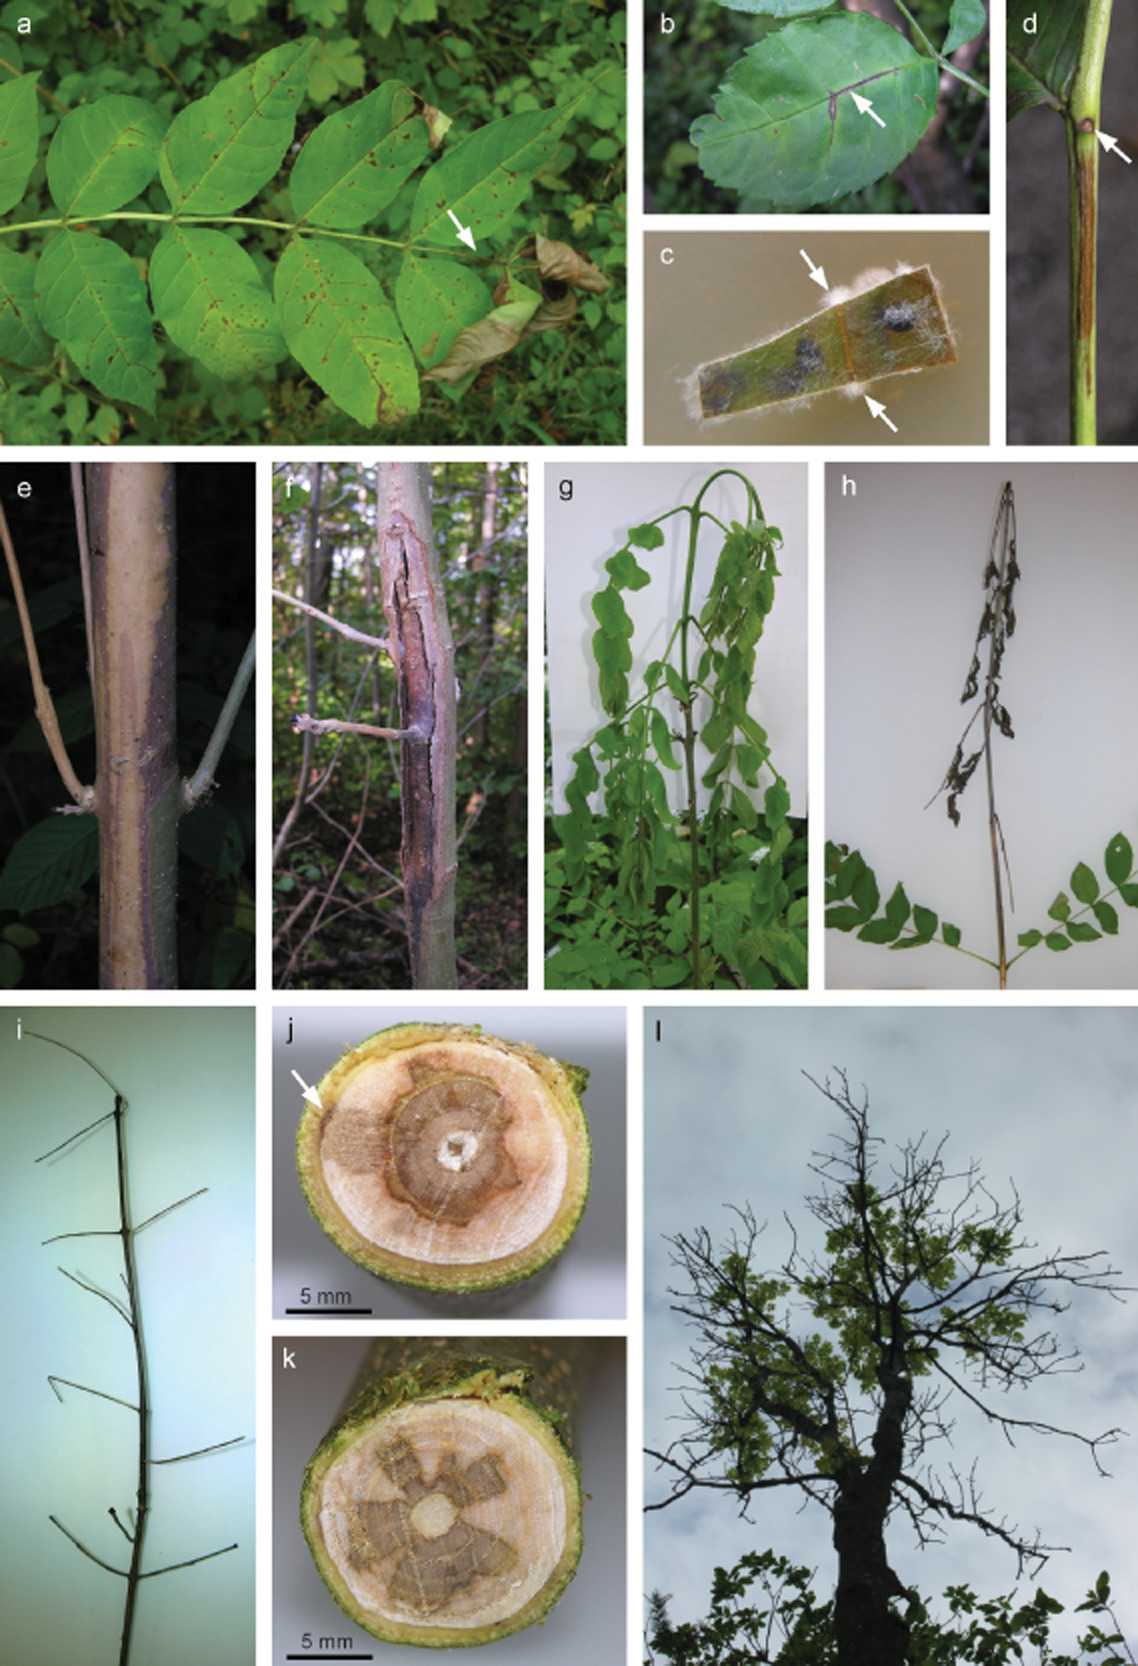
\includegraphics[scale=0.5]{chapter2/figures/gross2014.jpg}
    \caption{
    The symptoms of ash dieback, taken from the work of \cite{gross2014h}. 
    The pathogen \textit{H. fraxineus} infects the leaves of ash, leading to early onset wilting and desiccation. 
    The fungus then reproduces asexually, spreading through twigs, branches and eventually the xylem. 
    Symptoms include wilting, necrotic lesions, crown dieback and eventual mortality.}
    \label{fig:ash-deiback-symptoms}
\end{figure}

The pathogen HF is lethal to European ash (\textit{Fraxinus excelsior}) of all ages. 
Nevertheless, research has established that small young ash trees are more at risk,
and susceptibility declines with maturity. Surveys of ash stands conducted by \cite{marccais2017estimation} 
in Belgium recorded that after six years of infection, small young saplings died with $35\%$ mortality, 
whilst slightly larger ash ($<25 \mathrm{cm}$ in diameter) displayed mortality of $11\%$. 
In contrast only $3.2\%$ of large mature ash ($>25\mathrm{cm}$ in diameter) died.

Various sources of ash mortality data have been collected in different European countries;
in Germany, a forest stand of planted ash trees showed a $73\%$
mortality rate after five years \cite{langer2015ash} (as cited in a review
\cite{enderle2017ash}), while observations of ADB progression in Austria
suggest a low mortality rate of $5\%$ measured over a two-year window \cite{kessler2012dieback}. 
A study conducted at different sites throughout Great Britain suggests a time scale ranging between 
$3-15$ years of infected tree growth before death \cite{wylder2018evidence}.

In addition to age, ash survival also depends on the landscape. 
Landscape features and ADB progression were studied by \cite{https://doi.org/10.1111/1365-2745.13383} 
over a sample plot of size  $\mathrm{3.5km \times 6.5 km}$ in France; observations over two years
suggest that the surrounding landscape has little impact initially in $2012$. However, after pathogen establishment, 
later surveys in $2016$-$2018$ showed that landscape features play an essential role.
Among the results put forward by \cite{https://doi.org/10.1111/1365-2745.13383}, 
a highly abundant ash region increased the prevalence of collar canker and rachis symptoms in neighbouring ash.
In addition, the authors found that the influence of ADB decayed exponentially up to $200-300\mathrm{m}$ away from the high density source,
thus suggesting a density-dependency in ADB spread.

Modelling work suggests a myriad of environmental factors can also predict the
vulnerability of ash and subsequent spread of disease \cite{dal2014risk}.
Spatial regression analysis conducted by \cite{chumanova2019predicting} in the Czech Republic indicates that altitude 
is an important predictor of pathogen growth, which also support the strong negative temperature dependence observed by \cite{hauptman2013temperature}.

\newpage

\subsection{Life cycle and reproductive mode}
% WIKI: Hymenoscyphus fraxineus has two phases to its life-cycle: sexual and asexual.[9] The asexual stage (anamorph) grows in affected trees attacking the bark and encircling twigs and branches.[9] The sexual, reproductive stage, (teleomorph) grows during summer on ash petioles in the previous year's fallen leaves.[7] The ascospores are produced in asci and are transmitted by wind; this might explain the rapid spread of the fungus.[

The reproductive mode is intricate, and HF can infect hosts through the soil,
water, and air \cite{gross2012reproductive}; 
although, the primary natural driver of disease propagation is through wind-dispersal
during summertime sporulation. Sporulation typically occurs from June-September when 
fungal fruiting bodies on the previous litter-fall release ascospores \cite{grosdidier2018tracking, hietala2013invasive}.
Multiple ascospores sources can infect the same leaf \cite{gross2012reproductive}. 
Though the primary natural driver is wind, infection (and re-infection) of ash are also thought to be possible 
through the soil-borne mechanisms \cite{fones2016role}, albeit with low frequency.

Ash dieback is highly seasonal \cite{bengtsson2014seasonal} and follows a complex, yearly polycyclic infection cycle.
Infected ash hosts will shed their leaves in the autumn, proceeded by fungal fruiting bodies growing on the dead leaf litter until summertime.
In summer, fruiting body spores are wind-dispersed and continue the cycle by producing new secondary infections\textemdash 
together, the life cycle and symptom expressions are illustrated in Figure \ref{fig:ash-deiback-symptoms}.
It is interesting to note the cyclic similarities between yearly ADB infection/re-infection and the seasonal
infections due to crop rotations, e.g. \cite{tankam2020modelling}. 
Notwithstanding that infected crop removal usually coincides with harvest time instead of infected ash survival that can span years.

The life cycle of the fungus HF can be understood to have two well-differentiated reproductive modes, 
sexual and asexual\textemdash a common trait of phyla Ascomycota, or ascomycetes fungi \cite{hawker2016physiology}.
Initially, asexual spores (conidia) were hypothesised to only increase genetic variance and act as spermatia \cite{gross2014h};
however \cite{fones2016role} called this into question, suggesting instead that asexual reproduction of the pathogen 
may play a role in driving the pathogen spread. Despite the potentially significant claim put forward by \cite{fones2016role},
it has gained seemingly little traction, and the role of asexual reproduction is still not fully understood.

\newpage

\subsection{Dispersal}

In general, fungal spores have an efficient multi-scale wind-dispersal mechanism,
known to travel large distances \cite{golan2017long, wingen2013long, mundt2009aerial}
often described by power-law kernels, e.g. \cite{shaw2006assembling}.
From an epidemiological perspective, data on spore dispersal does not necessarily reflect the dynamics of new infections, 
as we cannot guarantee the availability of susceptible host material.
Even supposing available hosts, we cannot guarantee invasive spore colonisation.
However, studies on spore dispersal shed essential light on the spatial scale of ADB dispersal. 

Modern methods typically rely on `spore trapping' and real-time polymerase chain reaction (PRC) to study spores dispersal.
Data collected by \cite{chandelier2014detection} over three years using a (rotating arm) trapping system
and PRC amplification. The authors reported a $10\%$ spore trapping efficiency, and that most
dispersed ascospores remained within $50\mathrm{m}$ from the infectious source, with only a small number of spores exceeding 
distances beyond $50\mathrm{m}$. The work of \cite{chandelier2014detection} demonstrated the utility of novel PCR methods
to spore trap, but undesirably collected dispersal data over relatively small spatial scales.

Among the first landscape-scale fungal spore studies were conducted by \cite{long-range-dispersal}.
The authors focused on a comparable ascomycete fungus, \textit{Mycosphaerella fijiensis}, affecting banana plants.
Interestingly, \cite{long-range-dispersal} reported that asexual spore dispersal gradients extended 
a small distance $15\mathrm{m}$. As opposed to occasional, rare LDD in sexual (ascospore) dispersal up to $1000\mathrm{m}$.
Contrasting sexual and asexual spore dispersal was novel, and observing a small localised asexual dispersal gradient supports
the accepted idea that sexual dispersal in ADB is the dominant driver of disease spread.

Arguably the most comprehensive multi-scale study of ADB spore dispersal was performed by \cite{grosdidier2018tracking}.
In their paper, \cite{grosdidier2018tracking} tracked the local and landscape-level dispersal of ascospores
produced by \textit{H. fraxineus} in France.
The data collected relied on spore trapping and PRC; the reported trapping efficiency was $30–47\%$, marking an improvement over previous studies
e.g \cite{chandelier2014detection}. Most spores dispersal remained localised up to $50\mathrm{m}$ away from the inoculum source,
consistent with the results mentioned above put forward by \cite{chandelier2014detection}.
Nevertheless \cite{grosdidier2018tracking} set spore traps over much larger spatial scales ($\sim 100\mathrm{km}$),
subsequently detecting ADB spores $50-100\mathrm{km}$ ahead of the disease front.

Two dispersal kernels were used by \cite{grosdidier2018tracking}, a thin tailed Gaussian and an inverse 
power law of the forms:
\begin{equation}
    D(a, r) = \frac{1}{\pi a^2}\exp\big[-\frac{r^2}{a^2}\big]
    \label{eq:adb-ga}
\end{equation}
and
\begin{equation}
    D(a, r) = \frac{(b-1)(b-2)}{2\pi a^2}\big[ 1+ \frac{r}{a}\big]^{-b}
    \label{eq:geometric-invserse-power-law}
\end{equation}
where $a$ and $b$ are fitted parameters (for the Gaussian kernel, $a=\sqrt{2}\sigma$ with $\sigma$ being the standard deviation.). 
Equation \ref{eq:geometric-invserse-power-law} falls into the classical two-parameter geometric family of dispersal distributions.
The scale parameter is described by $a$ and the shape parameter by $b$. The mean dispersal distance described by Equation
\ref{eq:geometric-invserse-power-law} is  $\frac{2a}{b-3}$, and parameters $a$ and $b$ are valid for $a>0$ and $b>2$.

The functional form of Equation \ref{eq:geometric-invserse-power-law} is predicated on pollen dispersal studies,
as reviewed by \cite{nathan2012dispersal}. The tail of Equation \ref{eq:geometric-invserse-power-law} is 
particularly well suited to describe LDD events, as noted by \cite{https://doi.org/10.1111/j.1365-294X.2004.02100.x}
when describing the dispersal of pollen particulates. Moreover, a study by \cite{https://doi.org/10.1111/j.1365-294X.2006.03155.x}
used Equation \ref{eq:geometric-invserse-power-law} to model pollen-dispersal (and thus plant gene-flow) over landscape-level spatial scales. 
Presumably, the ability of Equation \ref{eq:geometric-invserse-power-law} to describe LDD, and the size similarity between pollen and fungi spores, 
motivated \cite{grosdidier2018tracking} to include it their field study. 
% A recent article published by \cite{golan2017long} presents an interesting system to 

\newpage

\subsection{Management and control}

Losing abundant ash populations could have dire consequences for several ecosystem functions, 
including nutrient recycling, food webs, and biodiversity.
As such, ADB presents a conservation challenge throughout Europe and Great Britain \cite{pautasso2013european}.
Moreover, under the rapid proliferation of ADB, various ash-dependent species risk extinction;
\cite{hultberg2020ash} identified $115$ at-risk (lichens, fungi, invertebrates, bryophytes/moss) species in Sweden that rely on ash.
Alarmingly, many of the ash-associated species identified by \cite{hultberg2020ash} also depend on elm species, which in turn face 
the fungal pathogen Dutch elm disease \cite{brasier1991ophiostoma}.

Given the ecological importance of ash in numerous temperate European forest types (e.g. floodplain, ravine, 
and lowland \cite{dobrowolska2011review}), management and pathogen control remain essential. The control of ash dieback
in a well-established focus of infestation, in both natural and artificial environments, is virtually impossible
\cite{havrdova2017environmental}, and it is already well recognised that ADB will eventually wipe out the vast 
majority of ash in Great Britain \cite{ash-dieback-costs}.

Controlling the spread of ash dieback reflects the spatial and temporal scale over which it spreads.
In particular, ADB fungal spores are thought to be able to jump between patches of ash,
even in the absence of susceptible hosts \cite{wingen2013long}.
However, LDD accounts for only a small minority of spore dispersal.
Furthermore, despite many notions of LDD, no unified LDD classification system exist, 
which led \cite{golan2017long} to propose a definition based on the distance traversed by the top $1\%$ of spores.

The long-term survival of ash depends on a small proportion of genetically resistant ash trees.
Despite many unpublished reports, genetic tolerance studies only began surfacing around a decade
after the widespread outbreak \cite{kjaer2012adaptive, stener2013clonal, mckinney2014ash}.
In particular, \cite{doi:10.1094/PHYTO-11-15-0284-R} showed the heritability of crown dieback and
collar-lesion symptom expression. In the three French provenances sampled,
\cite{doi:10.1094/PHYTO-11-15-0284-R} found no evidence for regional tolerance.
Presently, genetic tolerance is widely accepted \cite{havrdova2016differences, skovsgaard2017silvicultural},
and more recent work has focused on metabolomic tolerance classification,
profiling which metabolite markers correlate with resistance 
\cite{nemesio2020canditate, nemesio2020metabolomics, sidda2020diversity, chaudhary2020identification}.

A silvicultural system proposed by \cite{skovsgaard2017silvicultural} involves visually scoring severity based on crown dieback
and collar lesions. In this scheme, forest managers would inspect disease severity to record disease progression over time
and record genetically resistant trees to cultivate for future timber production. In addition, 
\cite{skovsgaard2017silvicultural} proposed that diseased forest stands should not be indiscriminately felled on account of high-value
tolerant individuals; this suggestion stands in contrast to the idea of a `cull radius', as alluded to by \cite{WEBIDEMICS}. 
In general, felling infected stands is ill-advised  \cite{chandelier2017ash}, except when infected hosts present a risk of uncontrolled 
and damaging tree-fall\textemdash as explained by \cite{ash-dieback-costs} when assessing the clean-up cost within Great Britain.

Following the establishment of genetic tolerance, numerous long-term preservation strategies 
rest on cultivating and replanting trees that exhibit low damage levels. Breeding 
programs in many European countries are currently underway, as reviewed by \cite{https://doi.org/10.1002/ppp3.10060}.
In the UK, the Living Tree Project (https://livingashproject.org.uk) aims to collate tolerant UK ash for future breeding.

% \cite{ash-tree2}
% - Approaches to conservation differ between forest and commercial ash stand \cite{skovsgaard2017silvicultural}. 
% - Among the control strategies, application of fungicide to infected biomass has been shown effective \cite{hauptman2015application}
% Among LDD human-mediated.
% - read me ->

% - statistical modelling work has shown the importance of environmental factors in the spread of disease \cite{dal2014risk, chumanova2019predicting}
% - the risk of spread.. was conduced by \cite{fellenor2019ash}....
% - \cite{dal2015epidemiology} un-published thesis